\documentclass{report}

\usepackage[colorlinks=true, pdfstartview=FitV, linkcolor=xkcdBlue, citecolor=xkcdRed, urlcolor=xkcdGreen]{hyperref}
\usepackage{graphicx}
\usepackage{color}
\usepackage{amsmath}
\usepackage{hyperref}
\usepackage{enumerate}
\usepackage{xcolor}
\usepackage{xkcdcolors}
\usepackage[]{algorithm2e}
\usepackage{float}


% \addtolength{\topmargin}{-.7in}
% \addtolength{\textheight}{.6in}
\usepackage[a4paper, left=1.80cm, right=1.80cm, top=2cm, bottom=2cm, bindingoffset=0cm]{geometry} 


\begin{document}


\Large
\textbf{AE4868-II (2025/2026) - Assignment 2} \\
\normalsize \\

\emph{\textbf{Last update: \today}}\\

Name: Ismael Gallo López \\

Student number: 6541356 \\

Github link: \textit{\href{https://github.com/ismaelgallolopez/numerical-astrodynamics-GALLO_LOPEZ_Ismael}{https://github.com/ismaelgallolopez/numerical-astrodynamics-GALLO\_LOPEZ\_Ismael}} \\

Time spent per exercise:
\begin{enumerate}
    \item 5 hours
    \item 8 hours
    \item 12 hours
    \item 10 hours

\end{enumerate} 

People you worked with (if none, state this):
\begin{itemize}
    \item Gemini 3
    \item Andreu Craus Vidal
    \item Daniel Pérez Trias
\end{itemize}

\clearpage

% \noindent\textit{Use this \LaTeX~file as a template for your report. All text that is not italic should be kept. All text that is italic, and all \ldots~should be removed and replaced by your answers. Only text that replaces \textbf{bold text} counts towards your line limit.}
% KC: bold text here > bold text?

\section*{Question 1}

% \textit{Insert figures} \\ 

\begin{figure}[H]
    \centering
    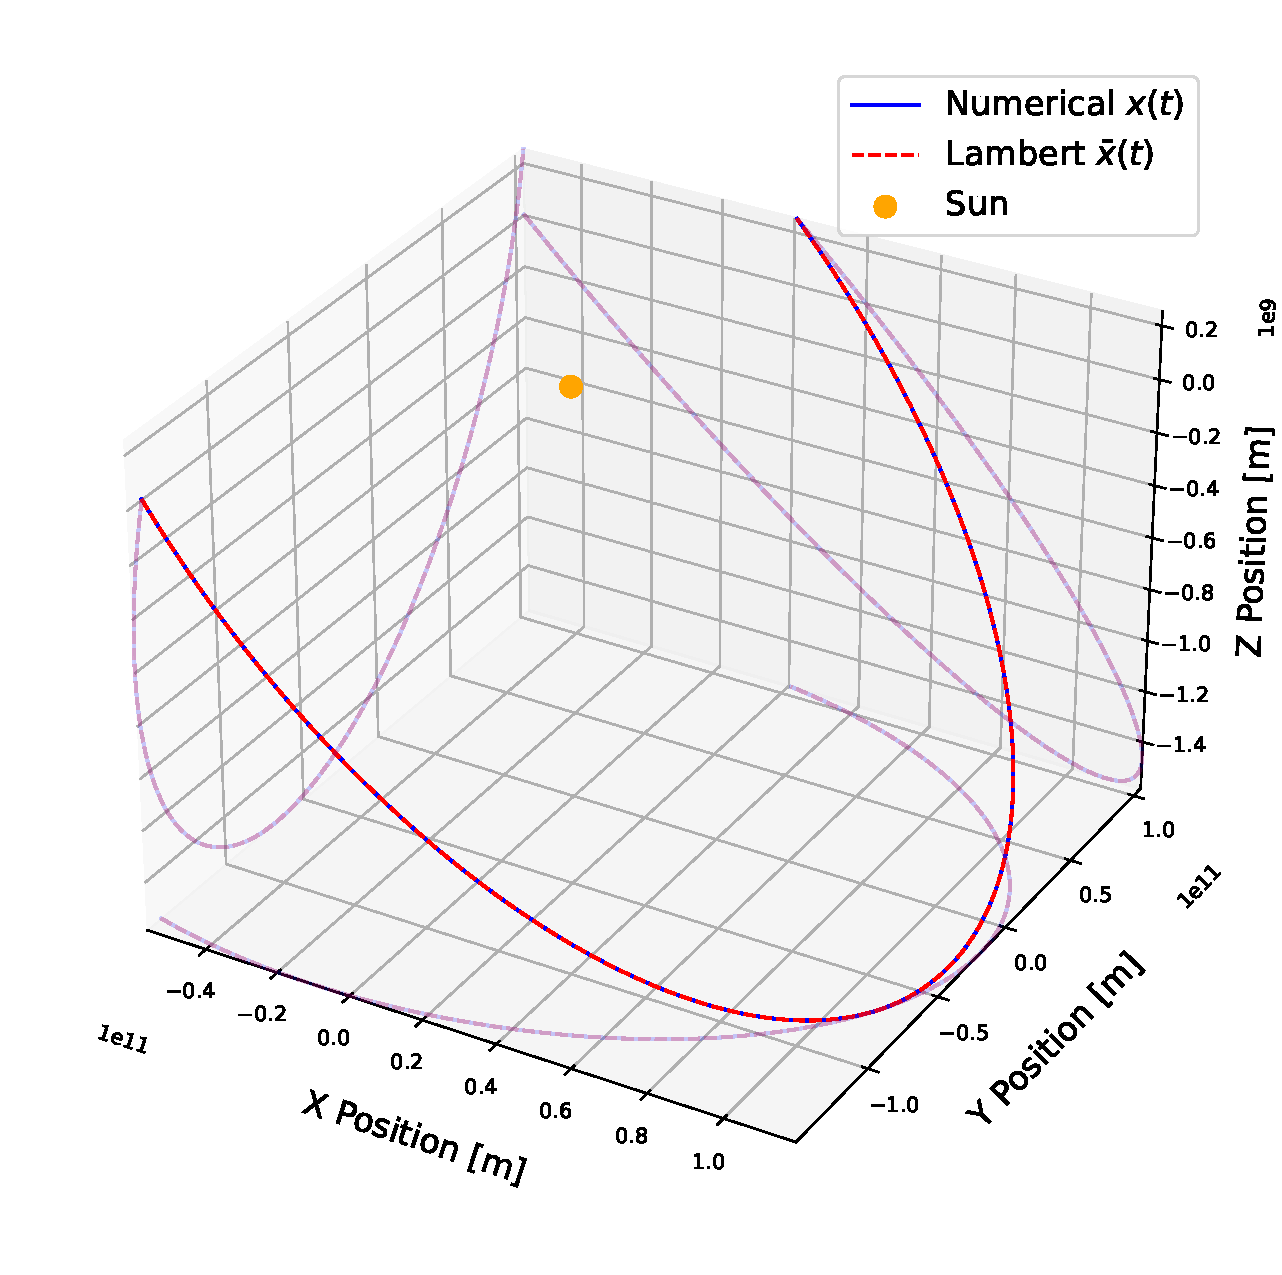
\includegraphics[width=0.7\textwidth]{../../figures/Q1_trajectory_3d.pdf}
    \caption{Trajectory of the spacecraft in the inertial frame.}
    \label{fig:Q1_trajectory_3d}
\end{figure}

\begin{figure}[H]
    \centering
    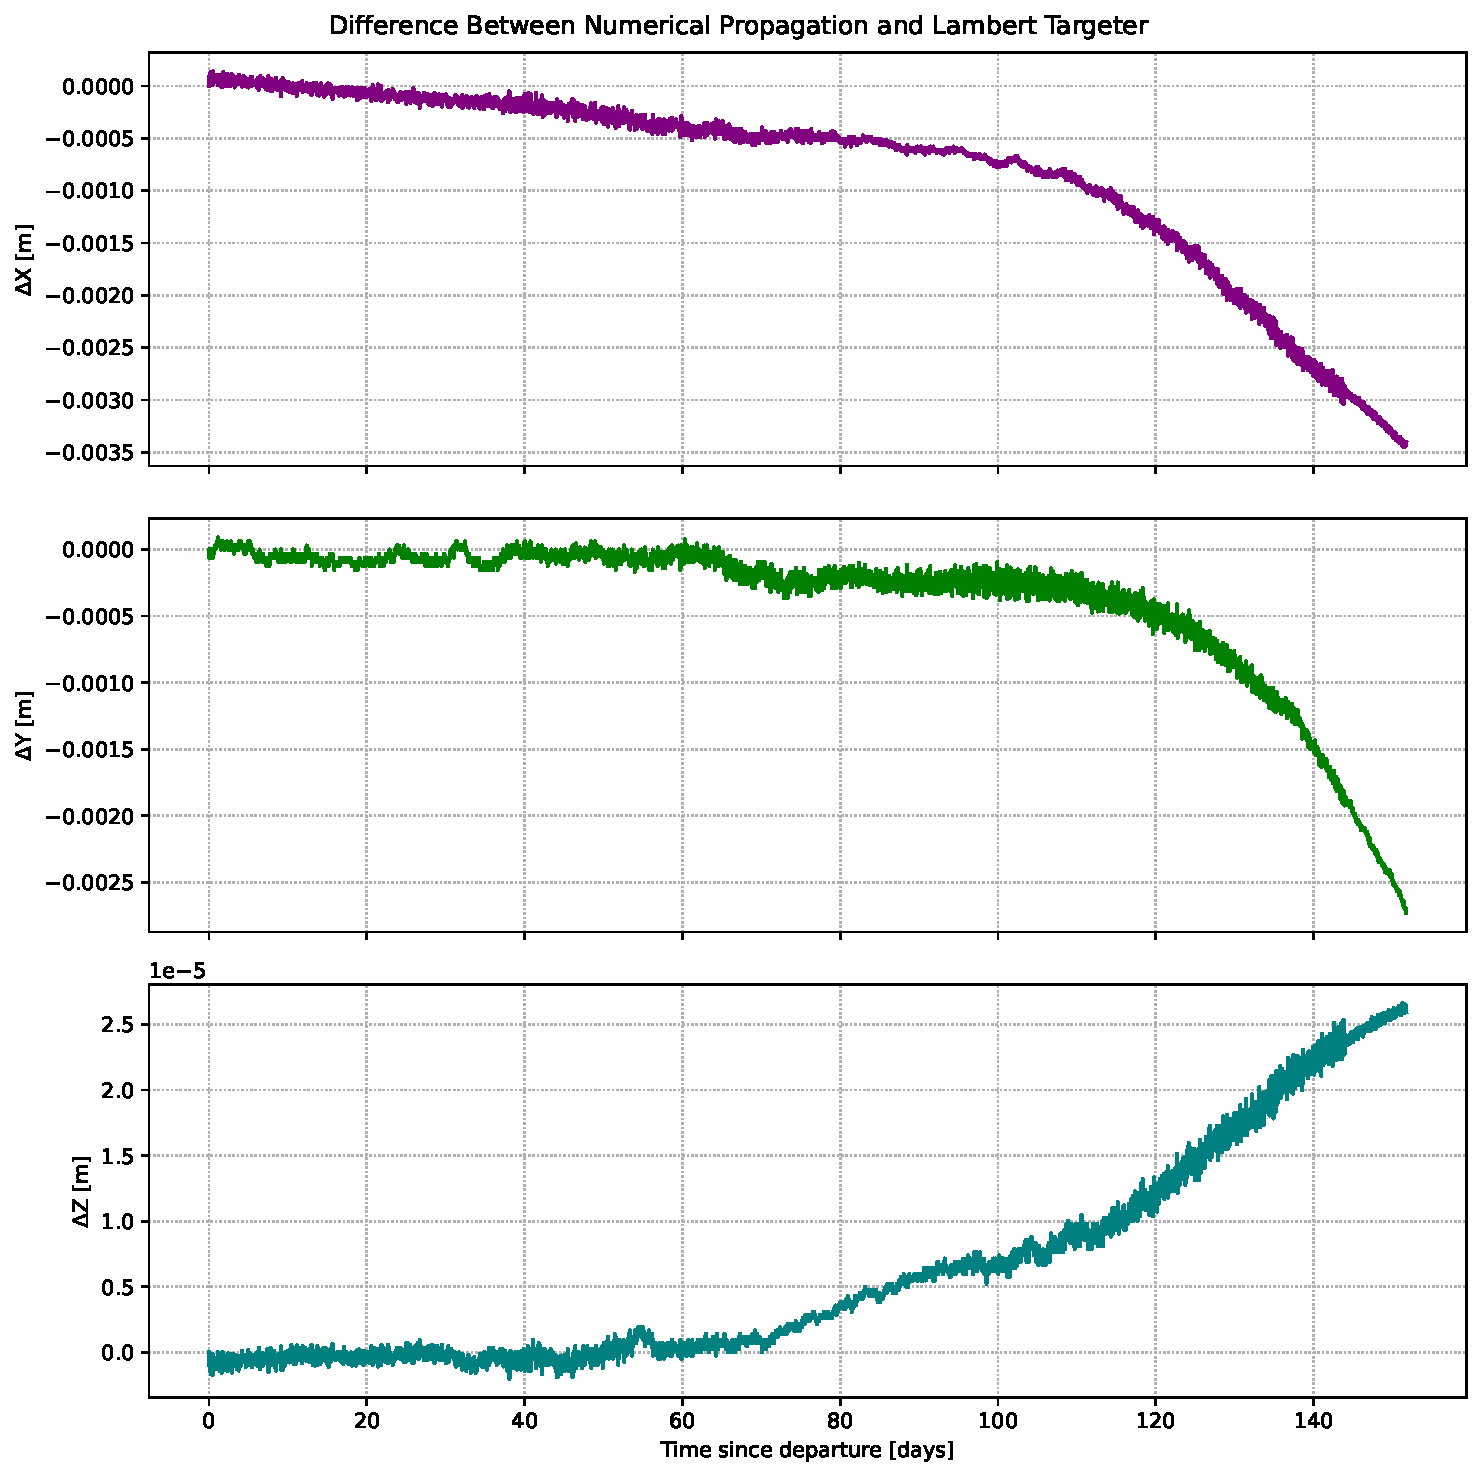
\includegraphics[width=0.8\textwidth]{../../figures/Q1_cartesian_differences.pdf}
    \caption{Differences between Cartesian coordinates between the numerical propagation and the analytical solution.}
    \label{fig:Q1_cartesian_differences}
\end{figure}

{{List of assumptions: }}\\
\begin{enumerate}
    % \item Assumption: ... ; True: yes/no  ;   \textbf{\textit{Explanation of why it is (not) true. If not true, explain whether it influences your propagation }}
    % \item Assumption: ... ; True: yes/no ;   \textbf{\textit{Explanation of why it is (not) true. If not true, explain whether it influences your propagation }}
    \item Only central body point mass exerts an acceleration; True; 
    
    Imposed by the environment.
    \item Start position w.r.t. central body is defined; True; 
    
    Idem.
    \item End position w.r.t. central body is defined; False; 
    
    The end position is a result of the integration.
    \item Time of flight is defined; True; 
    
    Is an input parameter of the propagation.
    \item Central body located at the origin (non-moving); False; 
    
    In reality, the Sun is not static, but at the scales of the problem, it has no effect.
    % \item At most a single revolution around central body (in this case); True; The propagation complies with that (see \autoref{fig:Q1_trajectory_3d}).
    % \item Prograde orbit; True; The propagation complies with that (see \autoref{fig:Q1_trajectory_3d}).
\end{enumerate}

\clearpage


\section*{Question 2}

\subsection*{a}
% \textit{Insert figure(s)}

\begin{figure}[H]
    \centering
    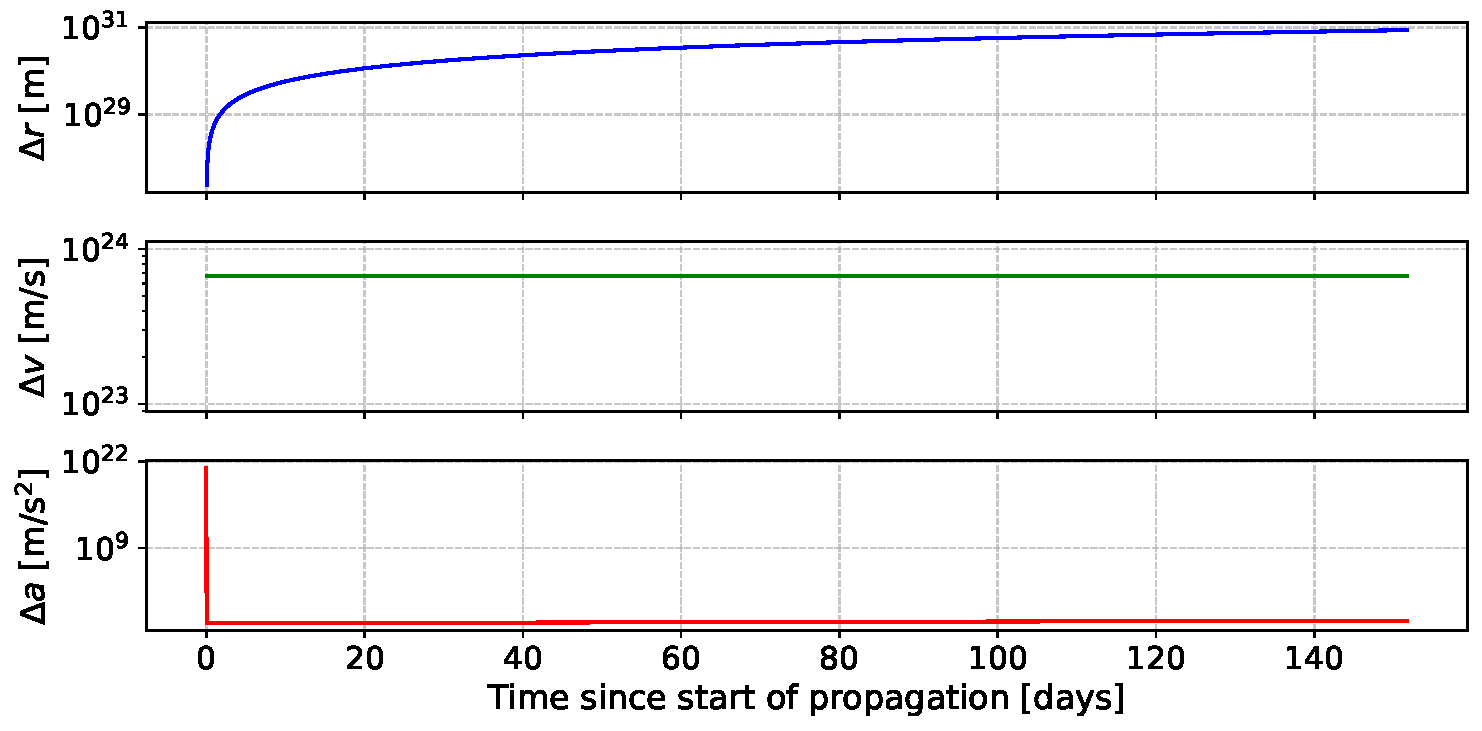
\includegraphics[width=0.8\textwidth]{../../figures/Q2_case_i_deviations.pdf}
    \caption{Differences between the numerical propagation and the environment-provided positions, case \textit{i}.}
    \label{fig:Q2_case_i_deviations}
\end{figure}

\begin{figure}[H]
    \centering
    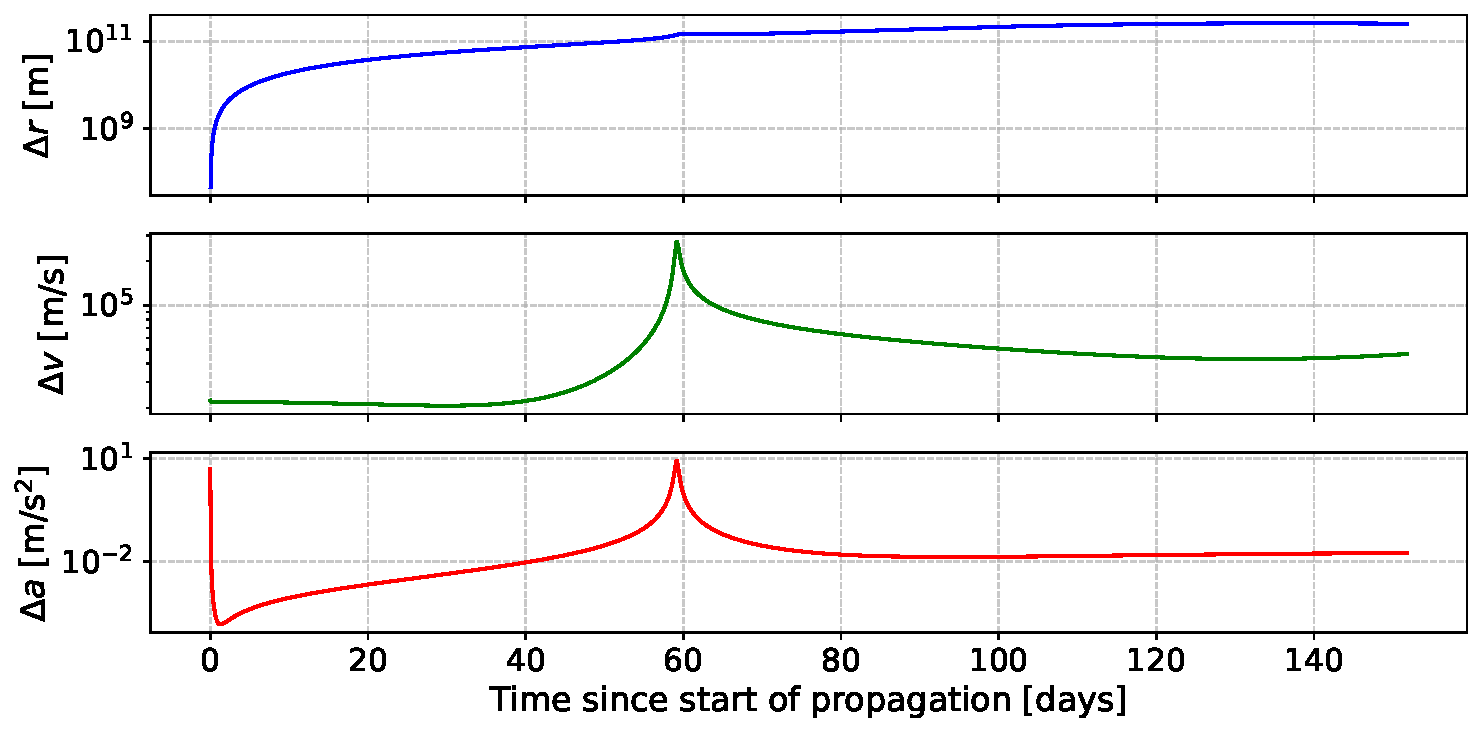
\includegraphics[width=0.8\textwidth]{../../figures/Q2_case_ii_deviations.pdf}
    \caption{Differences between the numerical propagation and the environment-provided positions, case \textit{ii}.}
    \label{fig:Q2_case_ii_deviations}
\end{figure}

\begin{figure}[H]   
    \centering
    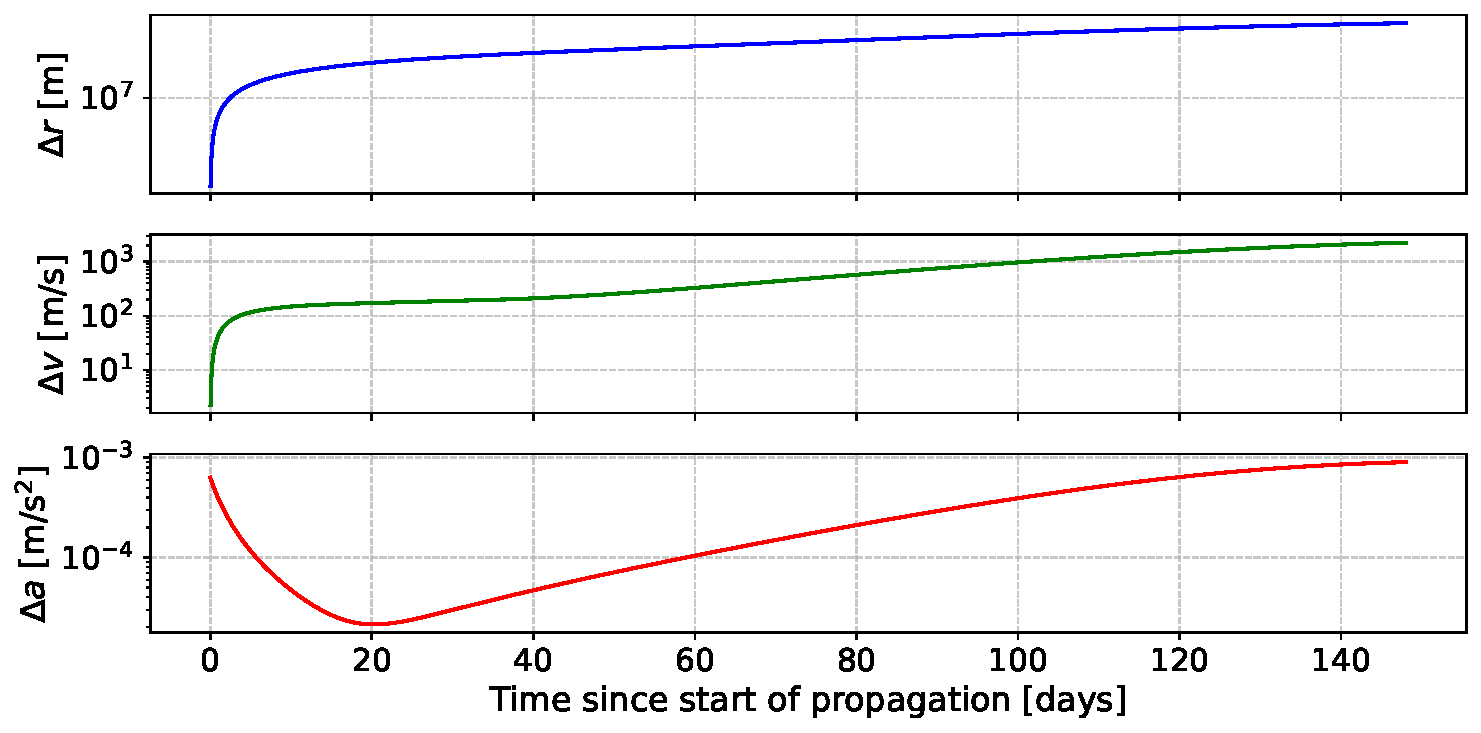
\includegraphics[width=0.8\textwidth]{../../figures/Q2_case_iii_deviations.pdf}
    \caption{Differences between the numerical propagation and the environment-provided positions, case \textit{iii}.}
    \label{fig:Q2_case_iii_deviations}
\end{figure}

\begin{figure}[H]
    \centering
    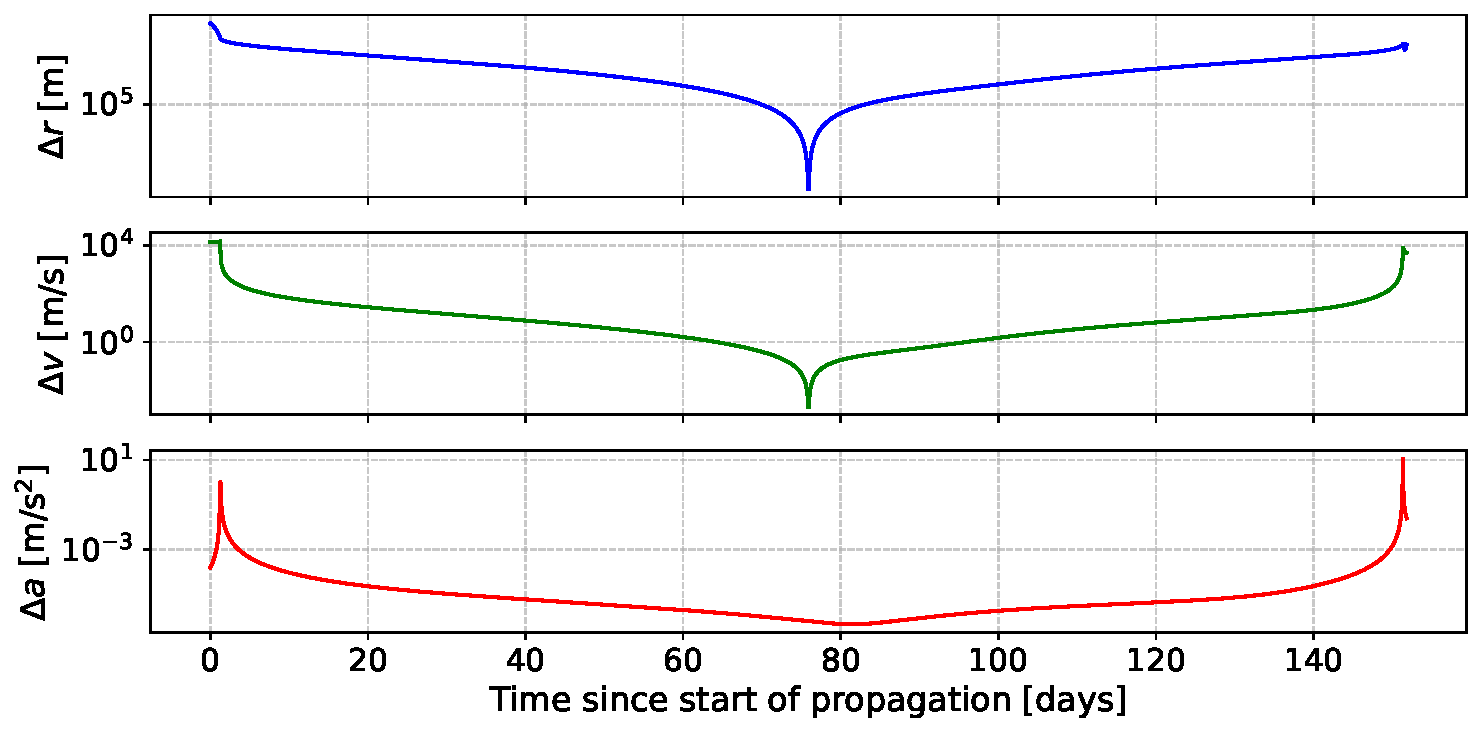
\includegraphics[width=0.8\textwidth]{../../figures/Q2_case_iv_m1000_deviations.pdf}
    \caption{Differences between the numerical propagation and the environment-provided positions, case \textit{iv}, with default mass of 1000 kg.}
    \label{fig:Q2_case_iv_m1000_deviations}
\end{figure}

\subsection*{b}
% \textbf{\textit{Provide reason that increasing buffer time generally reduces $\Delta r$ }}\\
% \textbf{\textit{Provide that propagating from arc center leads to lower $\Delta r$}}

Increasing buffer time avoids the ($\mathbf{a} \propto 1/r^2$) at the boundaries, drastically reducing numerical errors. 
This is evident when comparing initial accelerations: in case \textit{i} versus in case \textit{ii}. 
Additionally, propagating from the arc center halves the continuous integration time. 
Since dynamical errors grow non-linearly over time, splitting the integration duration significantly limits the maximum accumulated $\Delta r$ at the endpoints.

\subsection*{c}

% \textit{Insert figure(s)}\\
% \textit{Define linearity figure of merit (mathematically)}\\
% \textbf{\textit{Explain why figure of merit is a good one for this purpose}}\\
% \textbf{\textit{Answer question on linearity}}\\

Since the SRP perturbation scales as $a_{SRP} \propto 1/m$, the expected position deviations scale linearly with the difference in inverse masses relative to the baseline. 
This yields the following FoM\footnote{Figure of Merit}:

\begin{equation} \label{eq:fom}
    \text{FoM} = \frac{||\Delta \mathbf{r}_{250}||}{3 ||\Delta \mathbf{r}_{500}||}
\end{equation}

\begin{figure}[H]
    \centering
    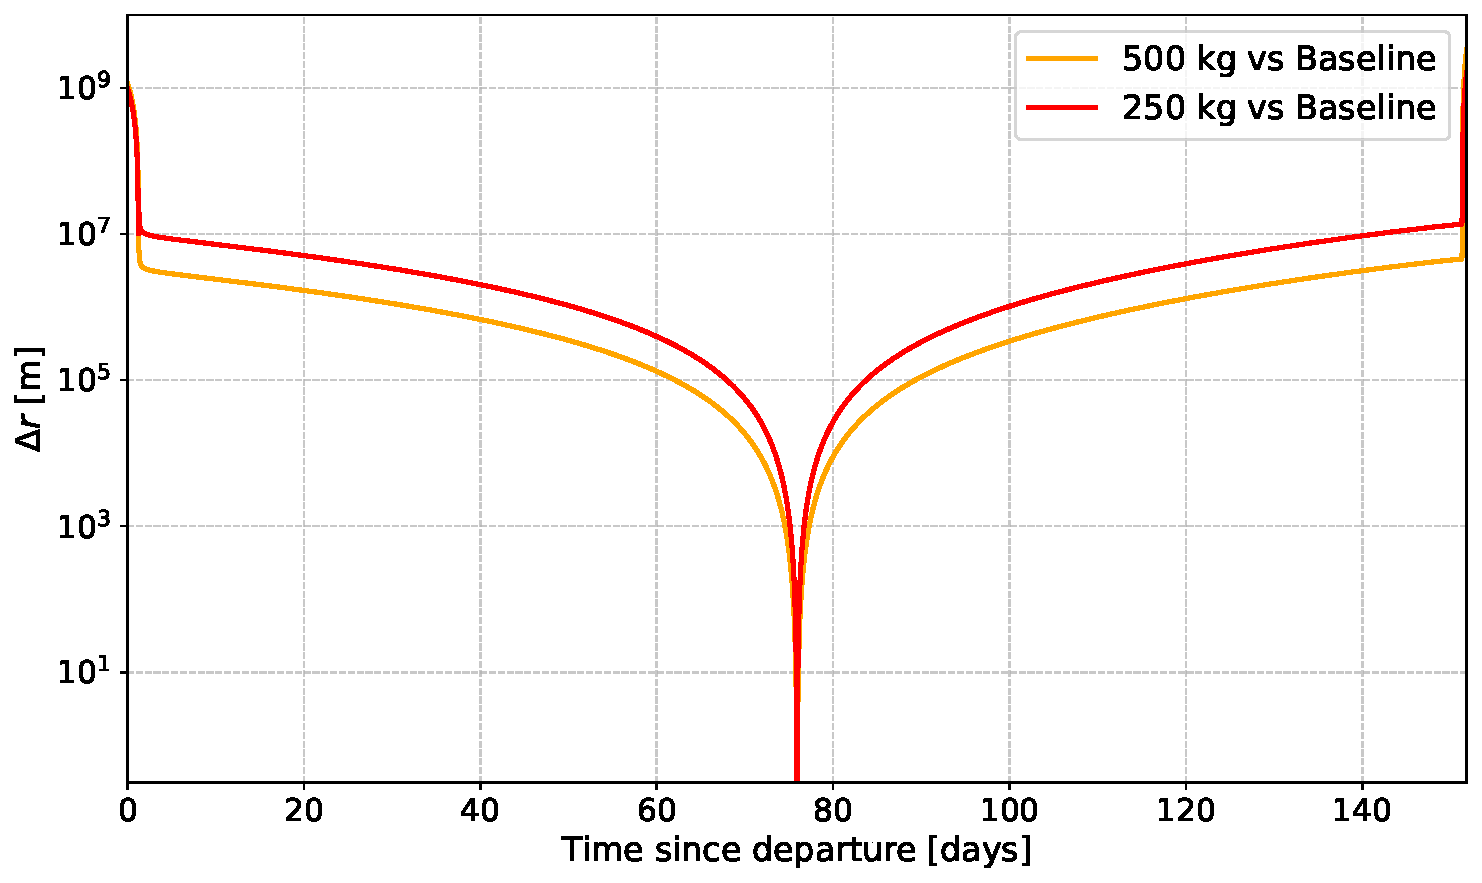
\includegraphics[width=0.8\textwidth]{../../figures/Q2_Mass_Position_Difference.pdf}
    \caption{Position differences for different spacecraft masses.}
    \label{fig:Q2_Mass_Position_Difference}
\end{figure}

\begin{figure}[H]
    \centering
    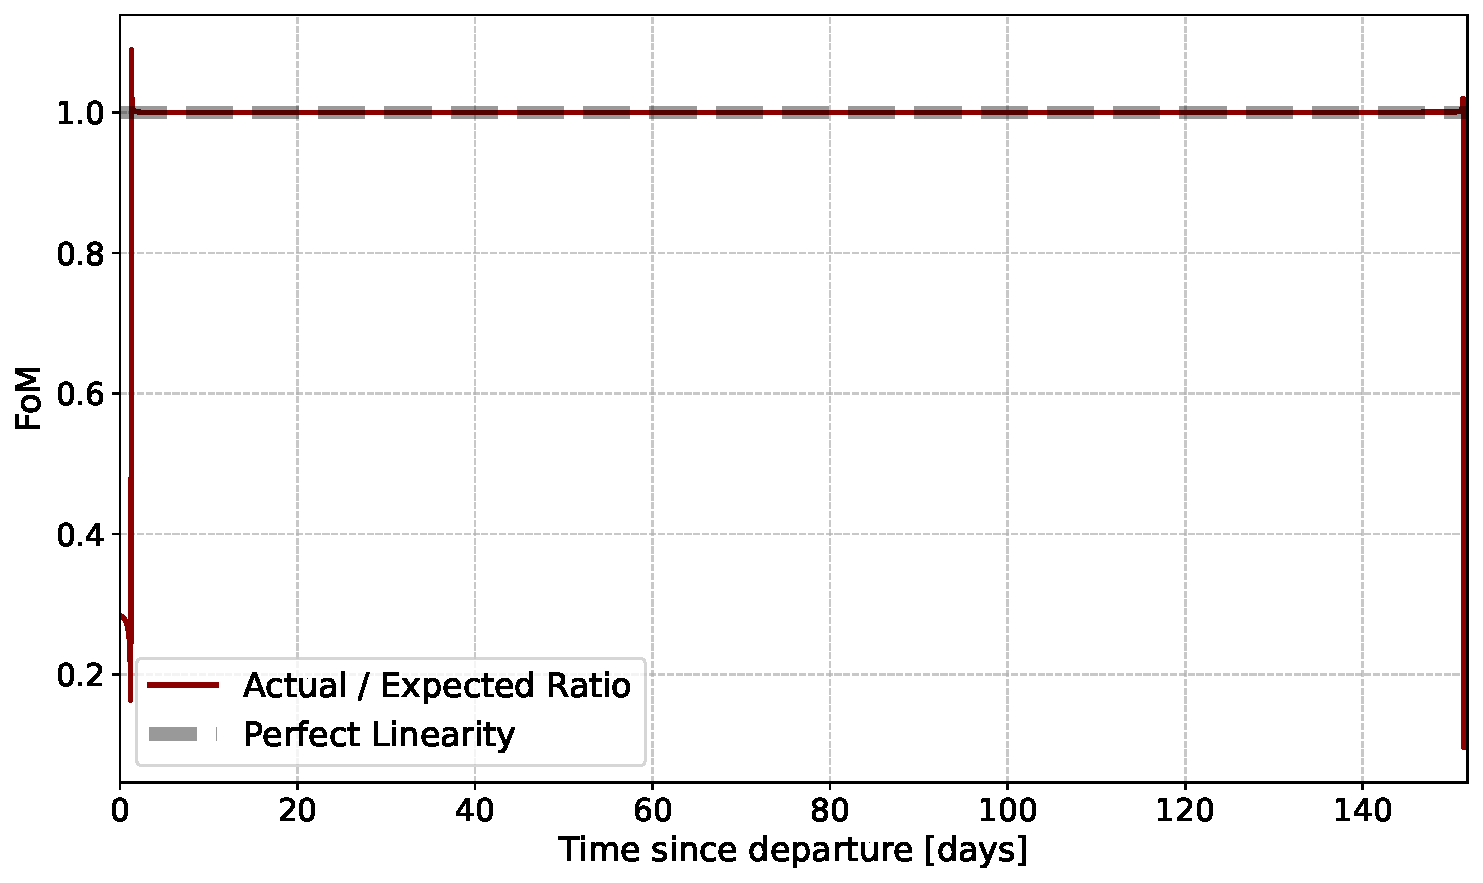
\includegraphics[width=0.8\textwidth]{../../figures/Q2_Figure_of_Merit.pdf}SS
    \caption{Figure of Merit (FoM) for spacecraft masses of 250 and 500 kg compared to the baseline (1000 kg).}
    \label{fig:Q2_Figure_of_Merit}
\end{figure}

The FoM remains near 1 for most of the transfer (\ref{fig:Q2_Figure_of_Merit}), indicating a highly linear response to mass variations. 
However, near the planetary boundaries, the FoM diverges from 1. 

\clearpage
\section*{Question 3}

\subsection*{a}
% \textit{Insert figure}
\begin{figure}[H]
    \centering
    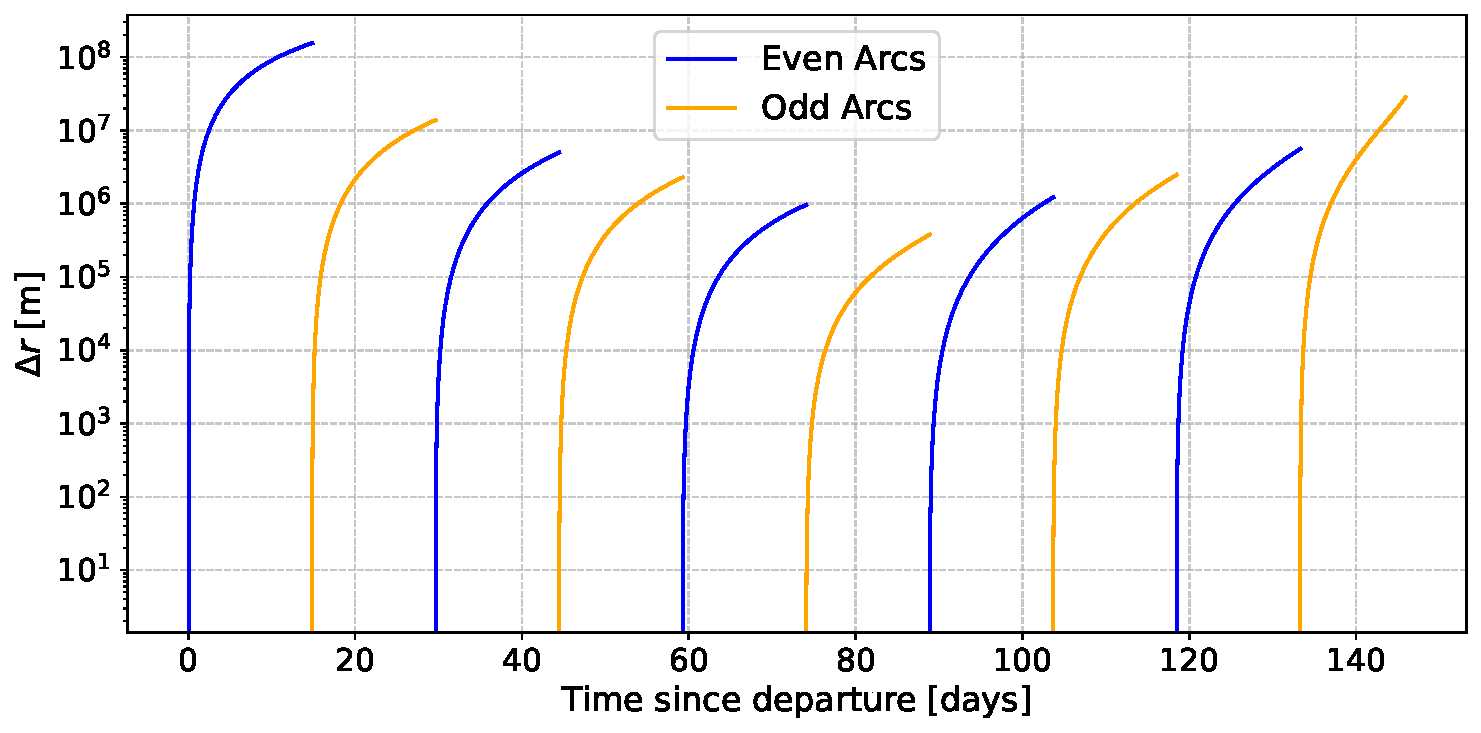
\includegraphics[width=0.8\textwidth]{../../figures/Q3_a_discontinuous_trajectory.pdf}
    \caption{Deviation of position for discontinuous propagated trajectory with respect to Lambert arc.}
    \label{fig:Q3_a_discontinuous_trajectory}
\end{figure}

\subsection*{b}
% \textit{Provide derivation/assumptions}\\
\begin{equation*}
    \Delta \textbf{x}_{i+1} = \mathbf{\Phi}_i (t_{i+1}, t_i) \Delta \textbf{x}_i ; \quad  \Delta \textbf{x}_i = \begin{pmatrix} \Delta \textbf{r}_i \\ \Delta \textbf{v}_i \end{pmatrix} ; \quad \mathbf{\Phi}_i (t_{i+1}, t_i) = \begin{bmatrix} \mathbf{\Phi}_{rr,i} & \mathbf{\Phi}_{rv,i} \\ \mathbf{\Phi}_{vr,i} & \mathbf{\Phi}_{vv,i} \end{bmatrix}
\end{equation*}

\begin{equation}
    \Delta \mathbf{r}_{i+1} = \mathbf{\Phi}_{rr,i} \Delta \mathbf{r}_i + \mathbf{\Phi}_{rv,i} \Delta \mathbf{v}_i \rightarrow \Delta \mathbf{r}_{i+1} - \mathbf{\Phi}_{rr,i} \Delta \mathbf{r}_i = \mathbf{\Phi}_{rv,i} \Delta \mathbf{v}_i
\end{equation}

Since the initial position is to be kept fixed, ($\Delta \mathbf{r}_i = \mathbf{0}$), and thus:
\begin{equation} \label{eq:linear_change_velocity}
    \Delta \mathbf{v}_i = \mathbf{\Phi}_{rv,i}^{-1} \Delta \mathbf{r}_{i+1}
\end{equation}

\subsection*{c}
% \textit{Insert figure}\\
\begin{figure}[H]
    \centering
    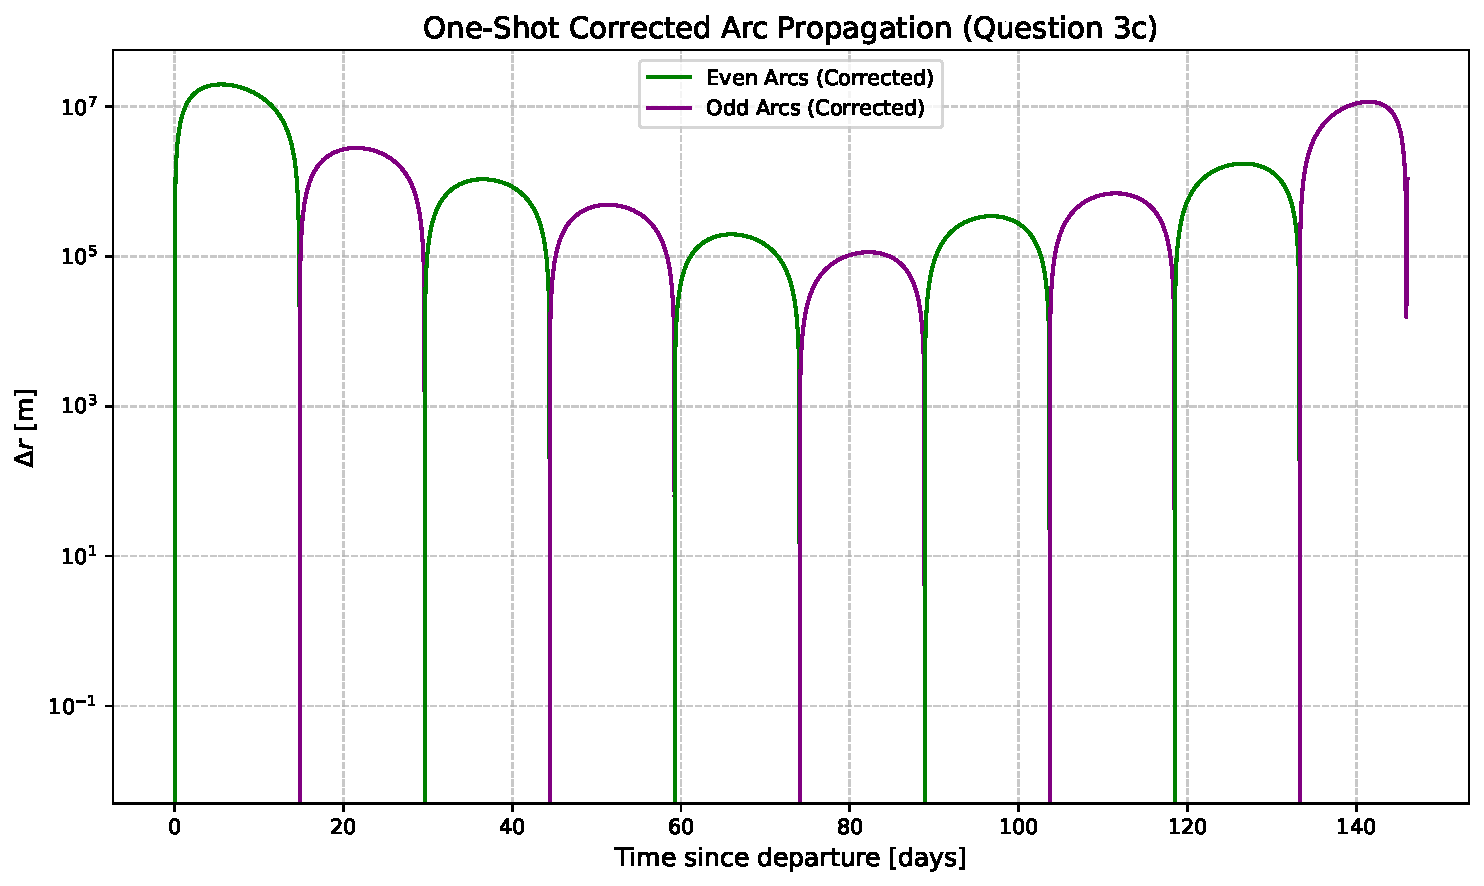
\includegraphics[width=0.8\textwidth]{../../figures/Q3_c_single_correction.pdf}
    \caption{Deviation of position for discontinuous propagated trajectory with respect to Lambert arc, corrected with the linearized equations formulation.}
    \label{fig:Q3_c_single_correction}
\end{figure}

\subsection*{d}
% \textit{Insert figure}\\
\begin{figure}[H]
    \centering
    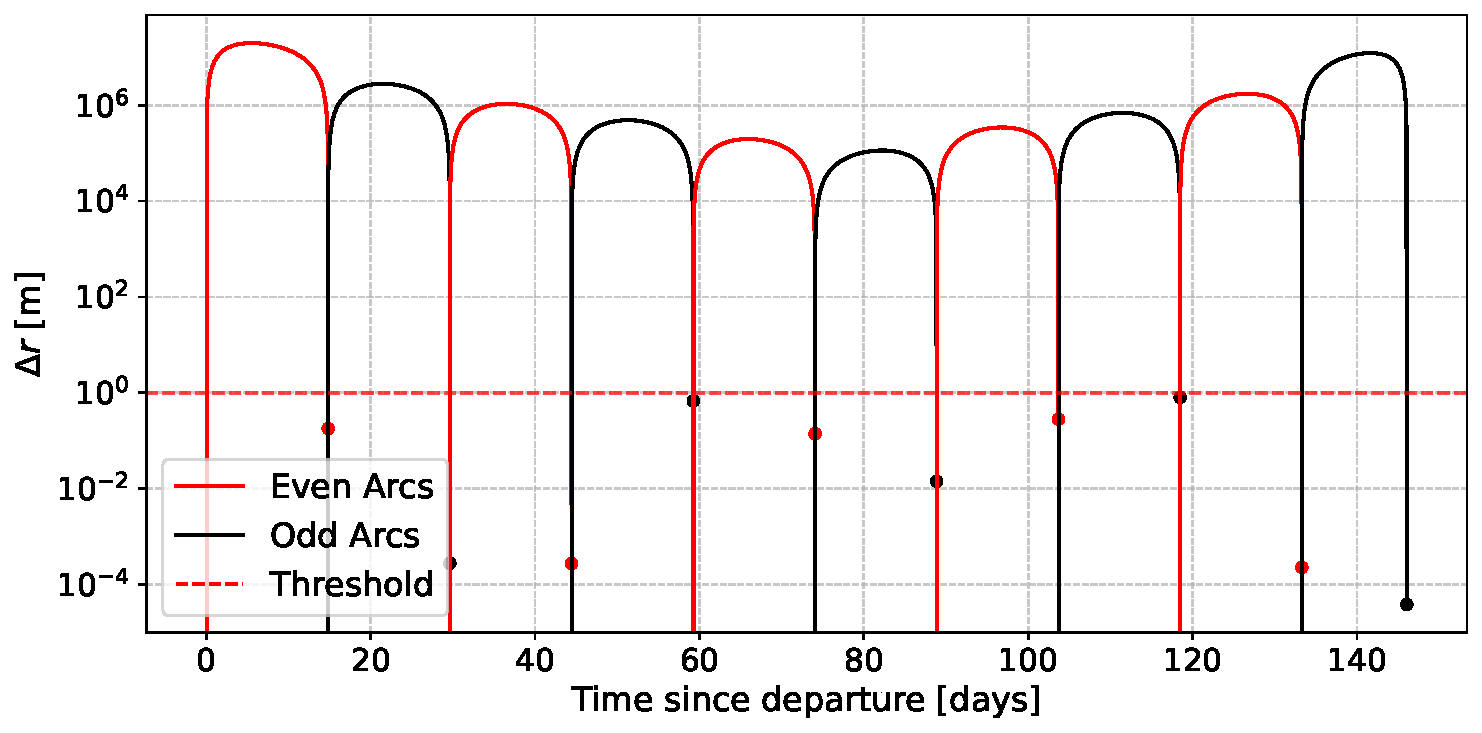
\includegraphics[width=0.8\textwidth]{../../figures/Q3_d_iterative_correction.pdf}
    \caption{Deviation of position for discontinuous propagated trajectory with respect to Lambert arc, for iterative modified final position.}
    \label{fig:Q3_d_iterative_correction}
\end{figure}

\begin{table}[H]
    \centering
    \caption{Number of iterations required for each arc to converge to within 1 m of Lambert arc.}
    \label{tab:Q3_d_convergence}
    \begin{tabular}{|c|c|c|c|c|c|c|c|c|c|c|}
        \hline
        Arc (\#) & 0 & 1 & 2 & 3 & 4 & 5 & 6 & 7 & 8 & 9 \\
        \hline
        Iterations to converge & 2 & 2 & 2 & 1 & 1 & 1 & 1 & 1 & 2 & 3 \\
        \hline
    \end{tabular}
\end{table}

% \textbf{\textit{Provide explanation why some arcs require more iterations than others.}}
From \ref{tab:Q3_d_convergence} it can be observed that the arcs in the middle of the propagation require less iterations than the middle ones.
The underlying reason is that the equation solved in \ref{fig:Q3_c_single_correction} (\ref{eq:linear_change_velocity}), is a linear approximation. 
Hence, in the extremes of the simulation, non-linearities are stronger and thus require to iterate further from the linear correction.

\subsection*{e}
% \textit{Provide derivation/assumptions}\\
% $\Delta V=$.... (equation)\\
% $\Delta V=$.... (number)

Assumptions:
\begin{enumerate}
    \item Maneuvers are impulsive and occur instantaneously at the start of each arc.
    \item Remaining position errors (< 1 m) between arcs are ignored for the $\Delta V$ budget.
\end{enumerate}

The total mission $\Delta V$ is the sum of the magnitude of the initial correction maneuver and the magnitudes of the velocity jumps at each of the $N-1$ intermediate nodes:
\begin{equation}
    \Delta V = \|\Delta \mathbf{v}_0\| + \sum_{i=0}^{N-2} \|\mathbf{v}_{i+1}(t_{0,i+1}) - \mathbf{v}_i(t_{f,i})\|
\end{equation}

Where:
\begin{itemize}
    \item $\|\Delta \mathbf{v}_0\|$ is the norm of the first impulsive correction at departure.
    \item $\mathbf{v}_i(t_{f,i})$ is the state vector velocity at the end of arc $i$.
    \item $\mathbf{v}_{i+1}(t_{0,i+1})$ is the state vector velocity at the start of arc $i+1$
\end{itemize}

\clearpage

\section*{Question 4}

\subsection*{a}
% \textit{Provide derivation/assumptions}\\
% $\mathbf{p}=...$

The full linearized relationship that links the changes in the initial state and system parameters to a change in the final state is:
\begin{equation} \label{eq:full_linear_params}
    \Delta \mathbf{x}(t_E) = \Phi(t_E, t_0)\Delta \mathbf{x}(t_0) + S(t_E)\mathbf{p}
\end{equation}

But the initial condition is that the numerical propagation starts at the same initial state as the Lambert arc: $\Delta \mathbf{x}(t_0) = \mathbf{0}$; hence \autoref{eq:full_linear_params} simplifies to:
\begin{equation}
    \Delta \mathbf{x}(t_E) = S(t_E)\mathbf{p}
\end{equation}

Isolating the parameter vector as done in \autoref{eq:linear_change_velocity}, the equation can be rewritten as:
\begin{equation}
    \mathbf{p} = S_r(t_E)^{-1} \Delta \mathbf{r}(t_E)
\end{equation}

\subsection*{b}
% \textit{Insert figure}\\
% The derived model is valid: \textbf{\textit{yes/no}}\\ 
% \textbf{\textit{Provide argumentation why you conclude your model is (not) valid.}}

The validity of the model developed in \textbf{a} is a little subjective. 
Even though the model reduces the final position deviation in comparison with the one shown in \autoref{fig:Q2_case_iii_deviations}, the position residual is still much greater than what would be an acceptable value, as can be seen in \autoref{fig:Q4_b_continuous_thrust_correction}. 
Because of the limitations of the linearized model, the correction is not sufficient to reduce the position error to an acceptable level, and thus, the model cannot be considered valid for this purpose.

\begin{figure}[H]
    \centering
    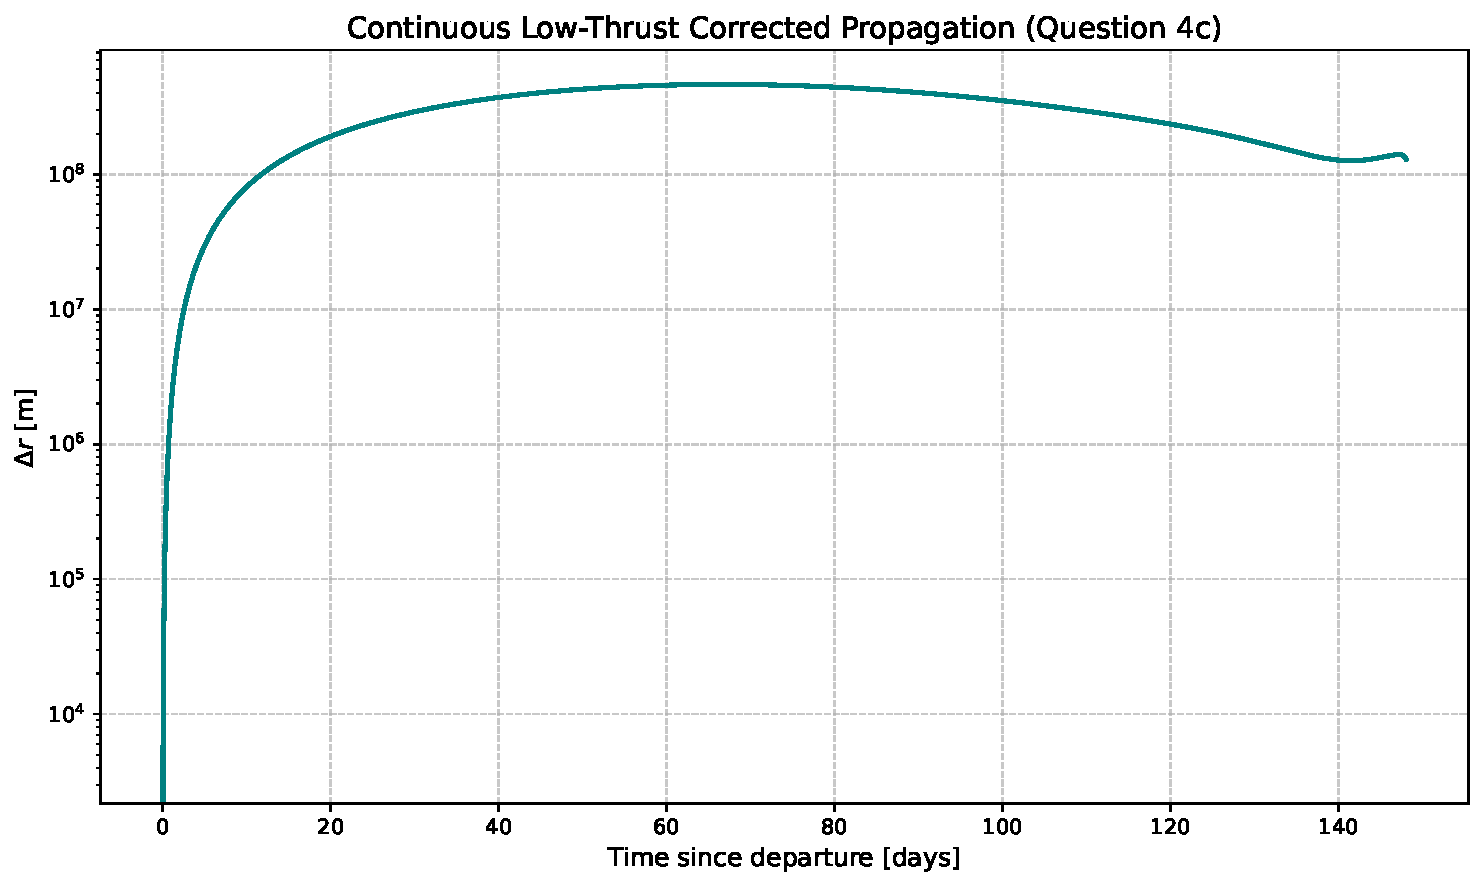
\includegraphics[width=0.8\textwidth]{../../figures/Q4_b_continuous_thrust_correction.pdf}
    \caption{Deviation of position for discontinuous propagated trajectory with respect to Lambert arc, for correction of system parameters.}
    \label{fig:Q4_b_continuous_thrust_correction}
\end{figure}

\subsection*{c.i}

% \textit{Provide derivation/assumptions}\\
% $\mathbf{p}_{2}=...$\\
% \textbf{\textit{Write out procedure for computing $\mathbf{p}_{2}$}}\\
% \begin{itemize}
%     \item $\mathbf{p}_{1}=...$ (from 4a)
%     \item ...
%     \item ...
%     \item $\mathbf{p}_{2}=...$ (from this question)
% \end{itemize}

One of the assumptions is that continuity in the state vector is imposed in the midpoint. 
Another assumption is that the system is enough non-linear to require an iterative solution search. 

For Arc 2, the change in the final position due to a change in the thrust vector is mapped by the position sensitivity matrix. 
At any iteration, the residual position error is $\Delta \mathbf{r}^{(k)} = \bar{\mathbf{r}}(t_E) - \mathbf{r}_2^{(k)}(t_E)$. 
We solve the linearized relation $\Delta \mathbf{r}^{(k)} = S_{r,2}(t_E) \Delta \mathbf{p}_2$ for the required thrust adjustment, and add it to our current guess.
\begin{equation}
    \mathbf{p}_{2}^{(k+1)} = \mathbf{p}_{2}^{(k)} + S_{r,2}(t_E)^{-1} \left( \bar{\mathbf{r}}(t_E) - \mathbf{r}_{2}^{(k)}(t_E) \right)
\end{equation}

Procedure for computing $\mathbf{p}_2$:
\begin{enumerate}
    \item $\mathbf{p}_{1}=\mathbf{p}^{(b)}$ (from \textbf{a})
    \item Propagate the dynamics of Arc 1 from $t_0$ to $t_{mid}$ using the Lambert initial state and the constant thrust $\mathbf{p}_1$. 
    \item Extract the final state $\mathbf{x}_1(t_{mid})$.
    \item Set the initial state of Arc 2 exactly to $\mathbf{x}_2(t_{mid}) = \mathbf{x}_1(t_{mid})$ and initialize the thrust guess as $\mathbf{p}_2^{(0)} = \mathbf{0}$.
    \item Iteratively propagate the variational equations for Arc 2 from $t_{mid}$ to $t_E$ to obtain the numerical position $\mathbf{r}_2^{(k)}(t_E)$ and the sensitivity matrix $S_{r,2}(t_E)$, applying the derived update equation for $\mathbf{p}_2$ until the boundary error $||\bar{\mathbf{r}}(t_E) - \mathbf{r}_2(t_E)|| < 1$ m.
    \item The final converged acceleration vector from the iterative loop $\rightarrow \mathbf{p}_{2}$.
\end{enumerate}

\subsection*{c.ii}

% \textbf{\textit{Answer question on value of $\mathbf{p}_{2}$}}

The value of $\mathbf{p}_2$ is almost identical to $\mathbf{p}^{(b)}$; both share roughly the same magnitude and point in the same direction (in each axis), with the radial component dominating. 
Because $\mathbf{p}^{(b)}$ was computed to completely eliminate the final position deviation under a linear assumption, applying it to Arc 1 corrects the vast majority of the trajectory. 
Consequently, $\mathbf{p}_2$ does not have to correct the massive initial Lambert discrepancy; it only needs to compensate for the minor non-linear residual errors accumulated during Arc 1.

\begin{table}[H]
    \centering
    \caption{Comparison of continuous thrust acceleration vectors for Arc 1 and Arc 2.}
    \renewcommand{\arraystretch}{1.3}
    \begin{tabular}{|l|c|c|c|c|}
        \hline
        \textbf{Parameter} & \textbf{Radial ($a_R$)} & \textbf{Along-track ($a_S$)} & \textbf{Cross-track ($a_W$)} & \textbf{Magnitude ($||\mathbf{p}||$)} \\
         & [m/s$^2$] & [m/s$^2$] & [m/s$^2$] & [m/s$^2$] \\
        \hline
        $\mathbf{p}_1$ (or $\mathbf{p}^{(b)}$) & $-4.7698 \times 10^{-5}$ & $-1.5101 \times 10^{-5}$ & $5.4854 \times 10^{-7}$ & $5.0035 \times 10^{-5}$ \\
        \hline
        $\mathbf{p}_2$ & $-4.7154 \times 10^{-5}$ & $-9.6424 \times 10^{-6}$ & $4.3066 \times 10^{-6}$ & $4.8322 \times 10^{-5}$ \\
        \hline
    \end{tabular}
    \label{tab:p1_vs_p2}
\end{table}

\subsection*{d.i}

% \textit{Insert figure(s)}

\begin{figure}[H]
    \centering
    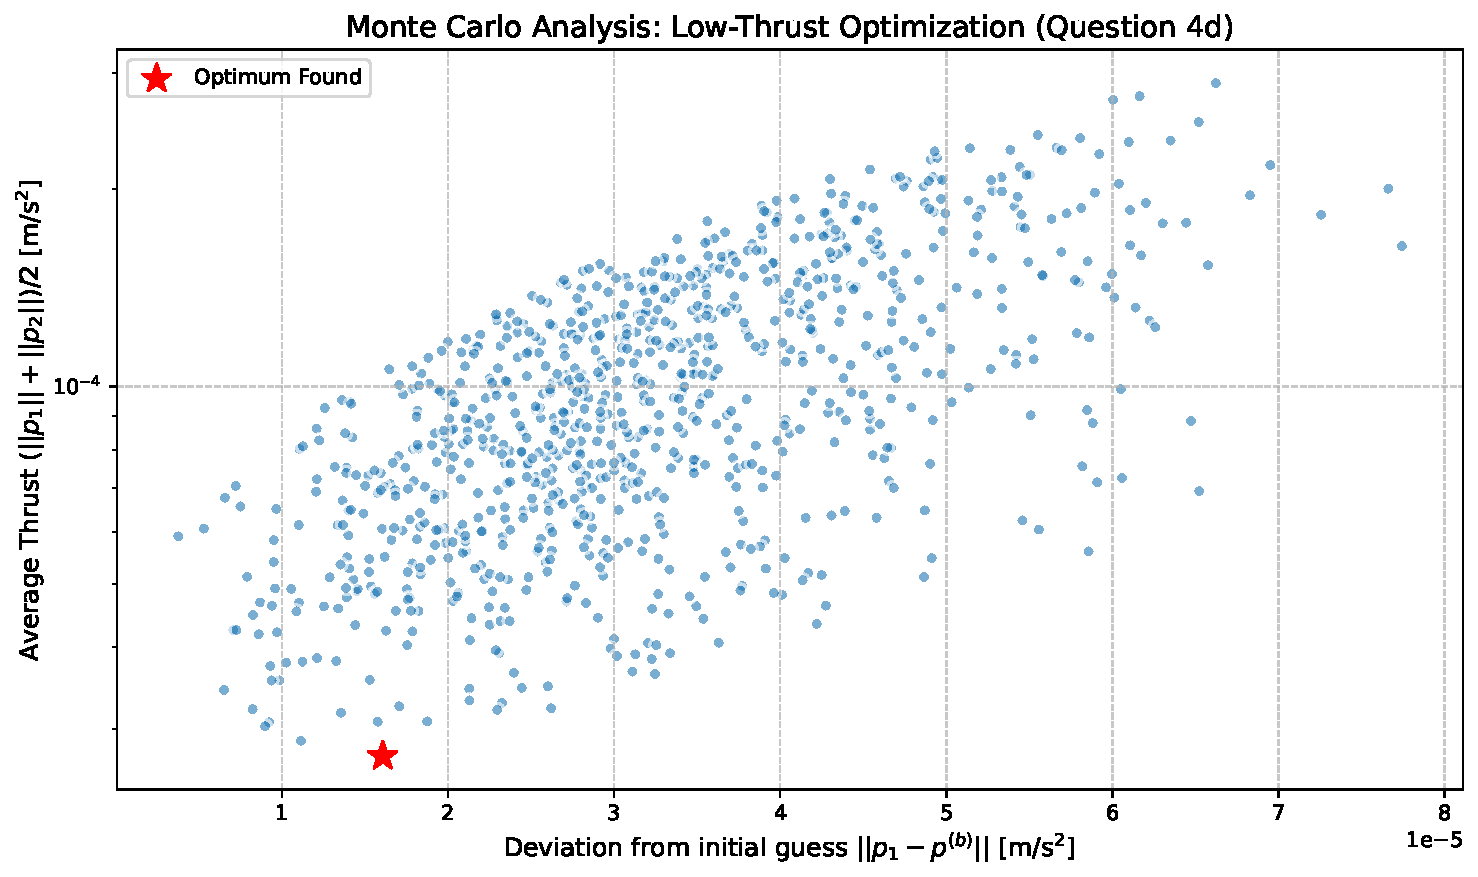
\includegraphics[width=0.8\textwidth]{../../figures/Q4_d_monte_carlo_scatter.pdf}
    \caption{Monte Carlo results for Arc 2.}
    \label{fig:Q4_d_monte_carlo_results}
\end{figure}

\begin{figure}[H]
    \centering
    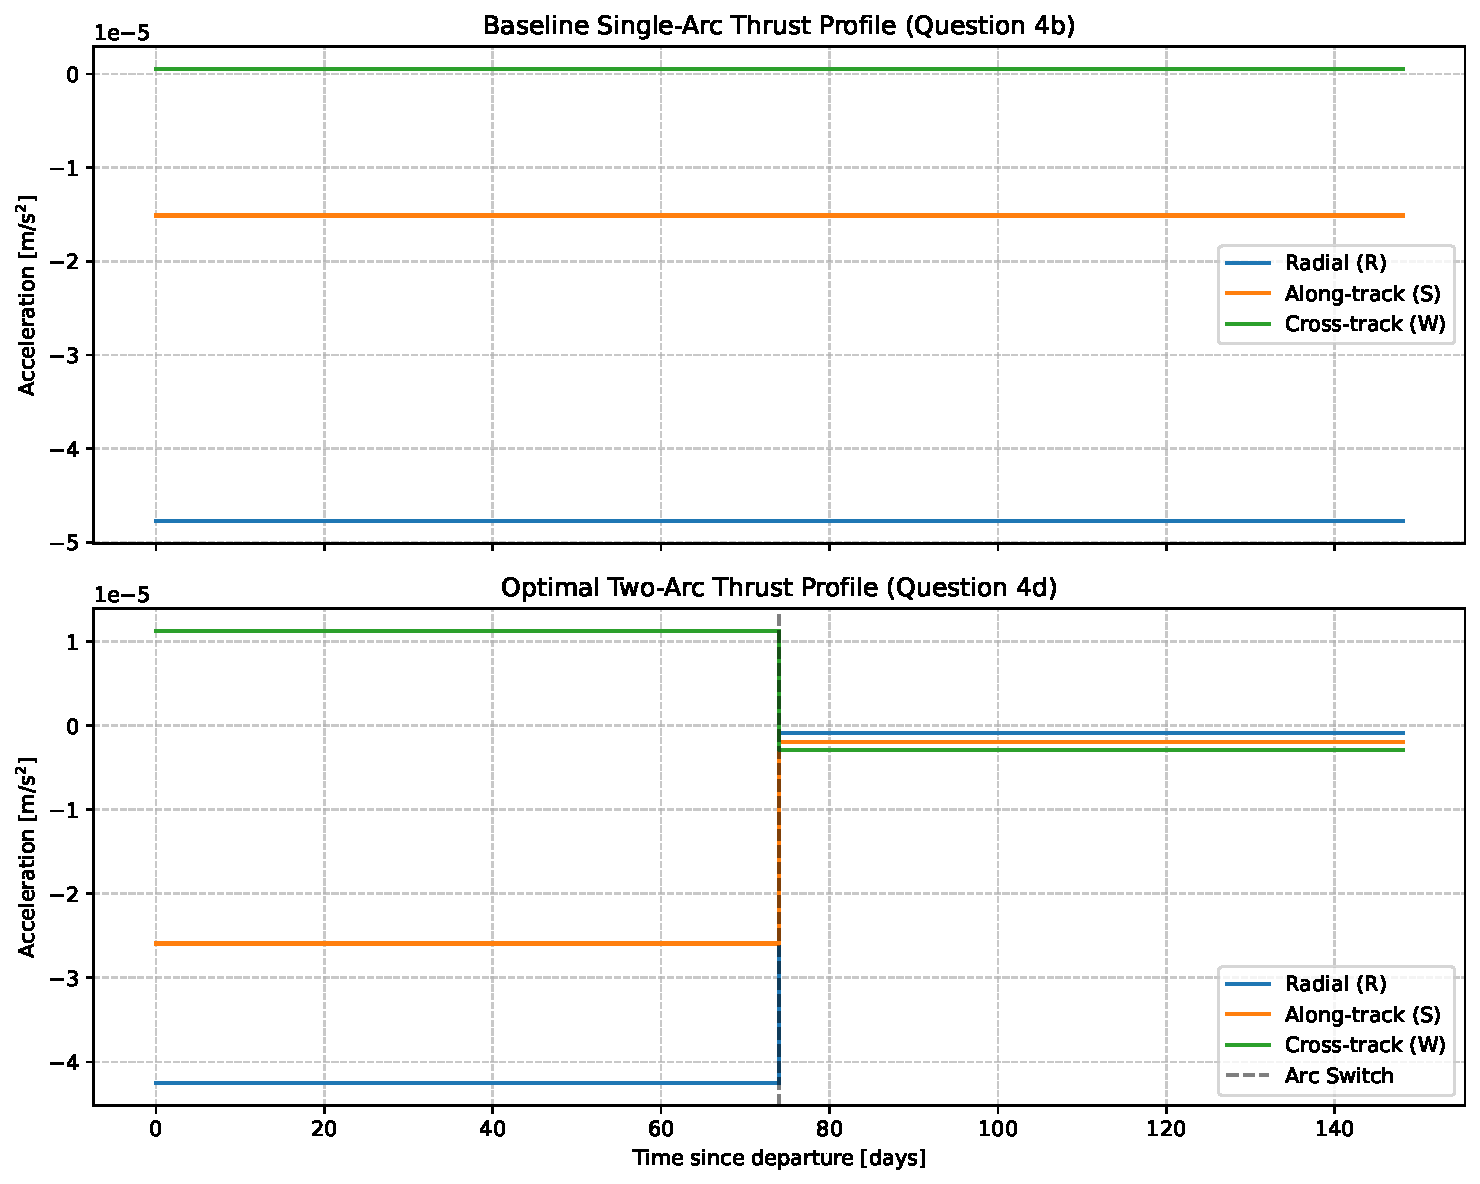
\includegraphics[width=0.8\textwidth]{../../figures/Q4_d_optimal_thrust_profile.pdf}
    \caption{Optimal thrust profile for Arc 2.}
    \label{fig:Q4_d_optimal_thrust_profile}
\end{figure}

\subsection*{d.ii}

% \textbf{\textit{Discuss observed behaviour of optimal thrust profile and answer the question}}

The optimal two-arc solution yields a lower average thrust because it exploits the varying orbital sensitivity along the trajectory. 
The rigid single-arc baseline forces a constant acceleration, often thrusting inefficiently against natural N-body gravity gradients. 
By allowing $\mathbf{p}_1$ to vary, the optimizer places the spacecraft into a dynamically favorable intermediate state at $t_{mid}$. 
This enables a highly efficient thrust reversal, braking inwards during Arc 1 and pushing outwards during Arc 2 (indicated by the sign flip in the $R$ and $S$ components), which minimizes the total corrective effort compared to a continuous brute-force push.

% \section*{Question 2}

% \subsection*{a}
% $\left(\mathbf{a}_{G,s}\right)_{G}=$ \ldots \\
% $\left(\mathbf{a}_{J,s}\right)_{G}=$ \ldots \\
% $\left(\mathbf{a}_{I,s}\right)_{G}=$ \ldots

% \subsection*{b}
% Positions from environment: \ldots \\
% Positions from numerical propagation: \ldots

% \subsection*{c.i}

% \textit{Insert figure}

% \subsection*{c.ii}

% $T_{\text{max,Io}}\approx\ldots$ hr \\
% $T_{\text{max,Sun}}\approx\ldots$ hr\\
% \textit{Insert figures, \textbf{descriptions}, \textit{etc.} to support your explanation}


% \subsection*{c.iii}

% $T_{\text{max,Io}}=K_{1} T_{\text{JUICE}} + K_{2} T_{I} + K_{3} T_{J}+\ldots.$ (\textit{replace right-hand side with relevant terms/coefficients}) \\
% $T_{\text{max,Sun}}=K_{1} T_{\text{JUICE}} + K_{2} T_{I} + K_{3} T_{J}+\ldots.$ (\textit{replace right-hand side with relevant terms/coefficients})

% \subsection*{c.iv}
% \textit{\textbf{Provide answer on physical reason for Io Period}} \\
% \textit{\textbf{Provide answer on physical reason for Sun Period}} \\
% \subsection*{c.v}
% \textit{Provide derivation, \textbf{and explain why the resulting equation leads to the expected conclusion (e.g. it explains the period found in c.iii)}}
% \clearpage

% \section*{Question 3}
% \subsection*{a}
% $\mathbf{a}_{\text{Aero}}=...$ \\
% $\mathbf{a}_{\text{SRP}}=...$ \\
% \textit{Insert figures validating acceleration implementation}.
% \textit{\textbf{Explain (briefly!) why the figures validate the implementation}}.

% \subsection*{b}
% \textit{Insert figures with accelerations in RSW frame.}
% \subsection*{c}
% Influence of acceleration formulation: \textit{\textbf{Provide answer}} \\
% Influence of definition of RSW frame: \textit{\textbf{Provide answer}} \\
% Influence of orbital geometry: \textit{\textbf{Provide answer}} \\
% \textit{\textbf{Brief summary of why these three points lead to the observed result}}.

% \subsection*{d.i}
% \textit{Insert figure}
% \subsection*{d.ii}
% Trend in $||\Delta \mathbf{r}_{G,s}(t)||$ for aerodynamics:~\textit{Provide answer} \\
% \textit{\textbf{Explanation for physical/mathematical reasons of the trend}}.

% \subsection*{d.iii}
% \textit{\textbf{Explanation for stronger relative influence of aerodynamic acceleration}}.
% \clearpage


% \section*{Question 4}
% \subsection*{a}
% ${\left(\mathbf{a}_{s}\right)_{J}}=\ldots$

% \subsection*{b}
% $\left(\mathbf{a}_{G,s}\right)_{J}=$ \ldots \\
% $\left(\mathbf{a}_{J,s}\right)_{J}=$ \ldots \\
% $\left(\mathbf{a}_{I,s}\right)_{J}=$ \ldots

% \subsection*{c}
% \textit{\textbf{Provide physical and mathematical explanation for the observed behavior}. Add figures, tables, equations, etc. to support your reasoning. Captions of these (including definition of terms in equations) do not count towards the line limit (within reason).}

% \subsection*{d}
% \textit{\textbf{Explain which model you think is most reliable and why}.}


\end{document}
